\par{The \emph{kernel} shown in listing \ref{private_memory_kernel} takes as a 
    base the previous kernel, but now it tries to use private memory to reuse 
    a complete row of matrix A to calculate every element of a row given to an specific
    \emph{work item}, this should bring a performance improvement due
    to the use of on chip memories in every of the devices studied, feature that 
    neihter of the previous \emph{kernels} implemented. Line \emph{9} of 
    listing \ref{private_memory_kernel} shows the copy of 
    elements of one row of matrix A from \emph{global memory} to
    \emph{private memory}, this allows the reuse of that data to calculate 
    a row of matrix C(resulting matrix) without going to \emph{global memory}
    again and again.} 

\par{Figure \ref{Rows} show that for the Xeon and Xeon Phi devices, 
    in terms of vectorization and degradation
    of performance when the number of \emph{work groups} start to decrease is the
    same as in the previous \emph{kernel}. Figures \ref{xeon} and \ref{phi} show
    a significative speedup between the previous \emph{kernel} and this one, 
    mostly because an increase in L1 hit ratio and vectorization intensity due to
    the reuse of data in A.}

\begin{figure}[!h]
    \centering
    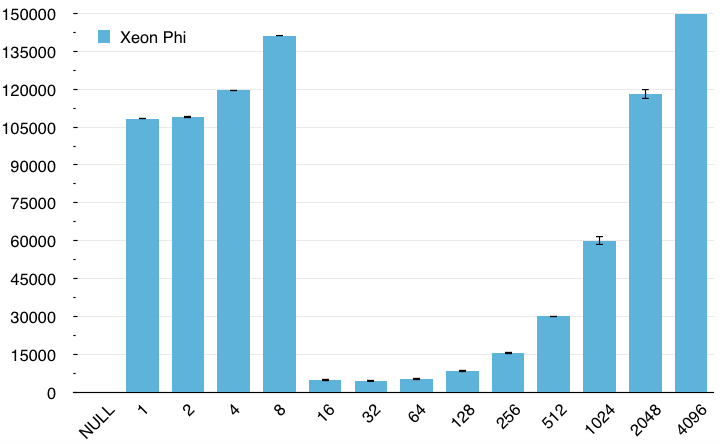
\includegraphics[width=0.49\textwidth]{figures/opt2_phi.png}
    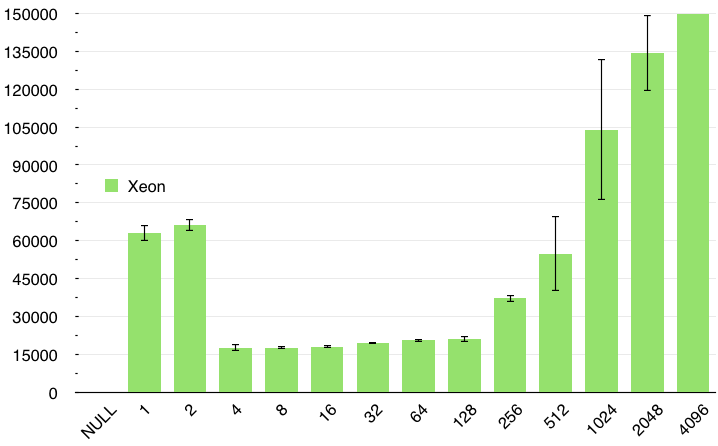
\includegraphics[width=0.49\textwidth]{figures/opt2_cpu.png}
    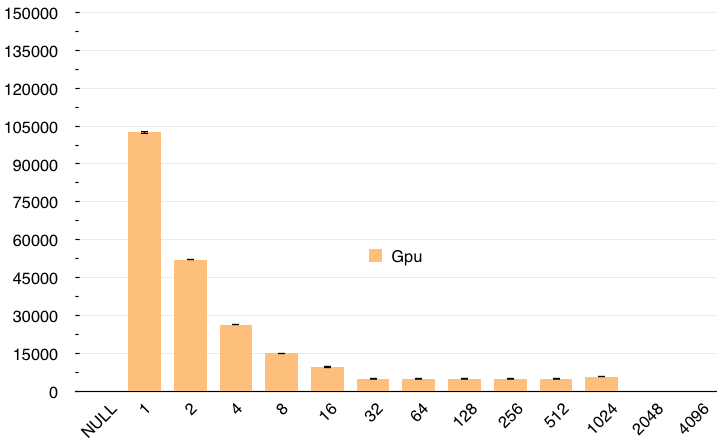
\includegraphics[width=0.49\textwidth]{figures/opt2_gpu.png}
    \caption{Row optimisation matrix multiplication in different architectures.}
    \label{Rows}
\end{figure}
    
\par{One interesting issue that we can observed looking at the assembly 
    code generated for the Xeon Phi, is that the 
    expensive gather operations from figure \ref{vtune_naive} in this 
    \emph{kernel} became very cheap in comparison as it can
    be seen in figure \ref{vtune_rows}, also this figure shows that the 
    \emph{vmovaps} \footnote{Moves packed single-precision 
    floating point values from aligned memory location to a destination 
    vector\cite{intrinsics}.} instruction became significant.}

\begin{figure}[!h]
    \centering
    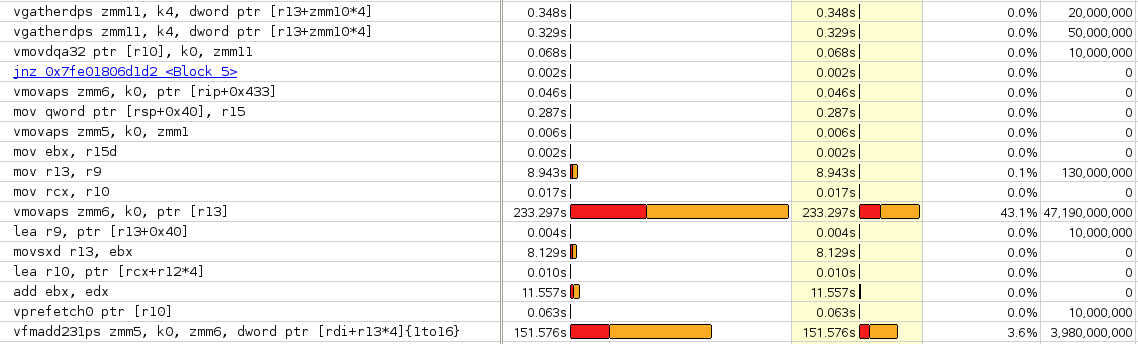
\includegraphics[width=0.9\textwidth]{figures/vtune_rows.png}
    \caption{Vtune analysis assembly code generated for the Xeon Phi.}
    \label{vtune_rows}
\end{figure}

\par{Figure \ref{Rows} shows also how the trend in the behaviour of the GPU
    changed from the previous \emph{kernel}. Performing a closer analysis of the
    new \emph{kernel} we can realise that the memory access pattern for copying
    the data from \emph{global memory} to \emph{priate memory} is strided, but
    happens only one time for every \emph{work item}. The intensive part of
    this kernel is performing the multiplications and accumulations, in this 
    part of the code(line \emph{14} listing \ref{private_memory_kernel}) 
    access to A and B have the same pattern. In both of them every thread in
    the warp access only one address of memory, this operation is perform using
    shuffle instructions which is very efficient, because  allows an exchange of
    32 bits between all threads in a warp\cite{broadcast}.}



\par{In this case the most performant architecture for this kernel is the 
    Xeon Phi by a very narrow margin as it can be seen \ref{RowRes}. Figures
    \ref{gpu}, \ref{phi} and \ref{xeon} show that in all the architectures this
    optimisations provided improvements in performance for the reasons explained
    previously.}

\begin{figure}[!h]
    \centering
    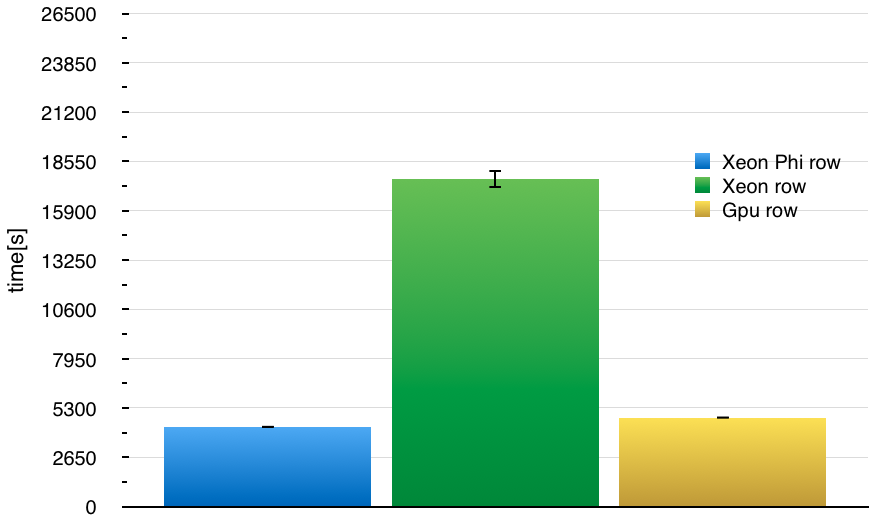
\includegraphics[width=0.49\textwidth]{figures/rowRes.png}
    \caption{Best case of row optimisation matrix multiplication in different architectures.}
    \label{RowRes}
\end{figure}



